%%%%%%%%%%%%%%%%%%%%%%%%%%%%%%%%%%%%%%%%%%%%%%%%%%%%%%%%%%%%%%%%%
% Capitulo 0 - introducao
%%%%%%%%%%%%%%%%%%%%%%%%%%%%%%%%%%%%%%%%%%%%%%%%%%%%%%%%%%%%%%%%%


\chapter{Introdu��o}
%\addcontentsline{toc}{chapter}{Introdu��o}

\vspace{-1cm} 
~
\begin{flushright}
\begin{minipage}[t]{6cm}
\footnotesize\textit{Bla bla bla}\\
\rule[0.01mm]{6cm}{0.01mm}\\
\end{minipage}
\end{flushright}
\vspace{0.5cm}


\nomenclature{ON}{Observatorio Nacional - MCT}


\begin{figure}[!htb]
     \centering
     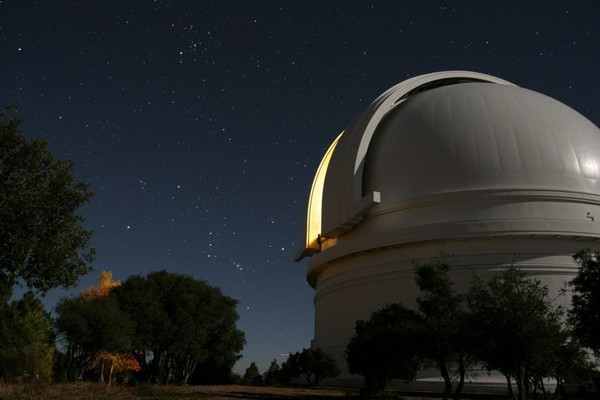
\includegraphics[scale=0.75]{figuras/palom1.jpg}
     \caption{Figura teste. O Caption que escreve aqui fica na figura}
     \label{O label que escreve aqui fica na lista de figuras.}
\end{figure}

